% ------------------------------------------------------------------------------
% TYPO3 Version 10.3 - What's New (German Version)
%
% @license	Creative Commons BY-NC-SA 3.0
% @link		https://typo3.org/help/documentation/whats-new/
% @language	German
% ------------------------------------------------------------------------------

\section{Backend User Interface}
\begin{frame}[fragile]
	\frametitle{Backend User Interface}

	\begin{center}\huge{Kapitel 1:}\end{center}
	\begin{center}\huge{\color{typo3darkgrey}\textbf{Backend User Interface}}\end{center}

\end{frame}

% ------------------------------------------------------------------------------
% Feature | 90333 | Dashboard

\begin{frame}[fragile]
	\frametitle{Backend User Interface}
	\framesubtitle{Dashboard (1)}

	Es wurde ein Dashboard eingeführt, das dem aktuell angemeldeten Backend-Benutzer wichtige Systeminformationen anzeigt.

	\begin{figure}
		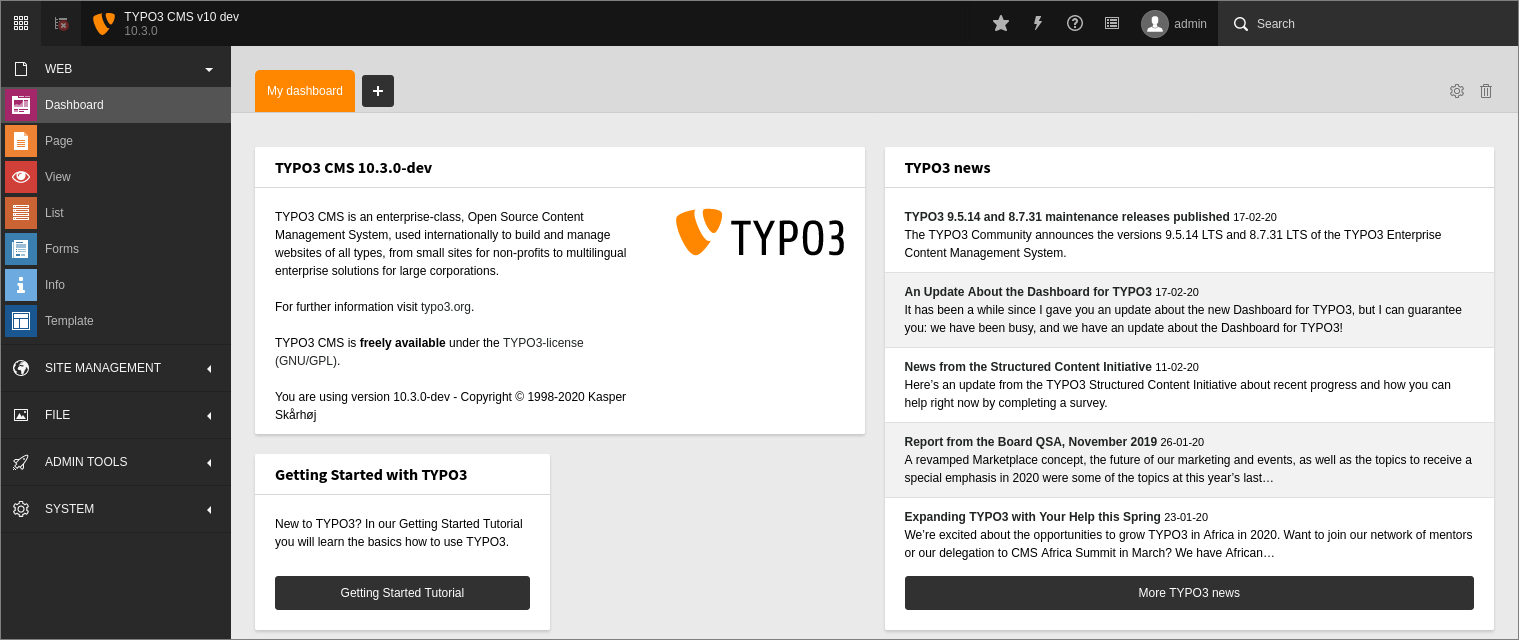
\includegraphics[width=1\linewidth]{BackendUserInterface/90333a-Dashboard.png}
	\end{figure}

\end{frame}

% ------------------------------------------------------------------------------
% Feature | 90333 | Dashboard

\begin{frame}[fragile]
	\frametitle{Backend User Interface}
	\framesubtitle{Dashboard (2)}

	Benutzer können ihre eigenen Dashboards erstellen und "Widgets" hinzufügen, entfernen und neu anordnen.
	Entwickler können benutzerdefinierte Widgets als Erweiterungen erstellen.

	\begin{figure}
		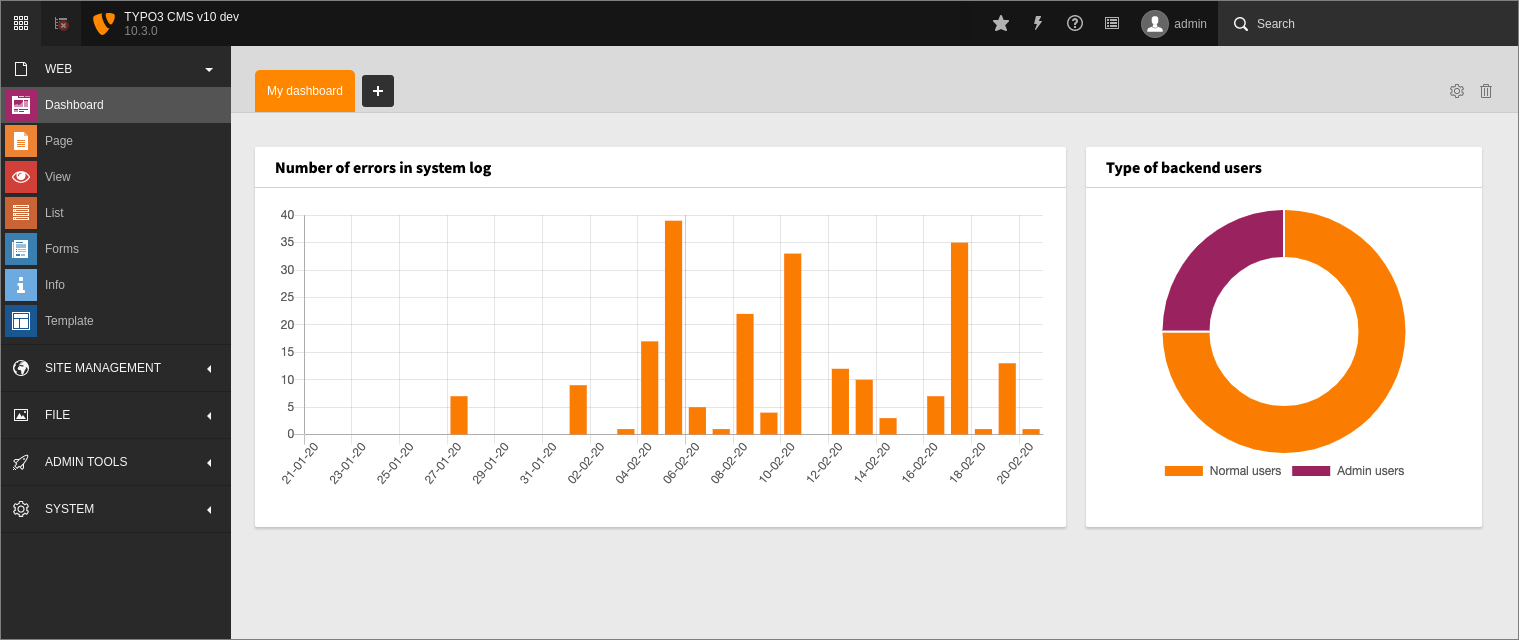
\includegraphics[width=1\linewidth]{BackendUserInterface/90333b-Dashboard.png}
	\end{figure}

\end{frame}

% ------------------------------------------------------------------------------
% Feature | 89513 | Provide password recovery for backend users
%
%\begin{frame}[fragile]
%	\frametitle{Backend User Interface}
%	\framesubtitle{Password Recovery}
%
%	Backend users can now reset their passwords in case they have forgotten it.
%
%	\begin{figure}
%		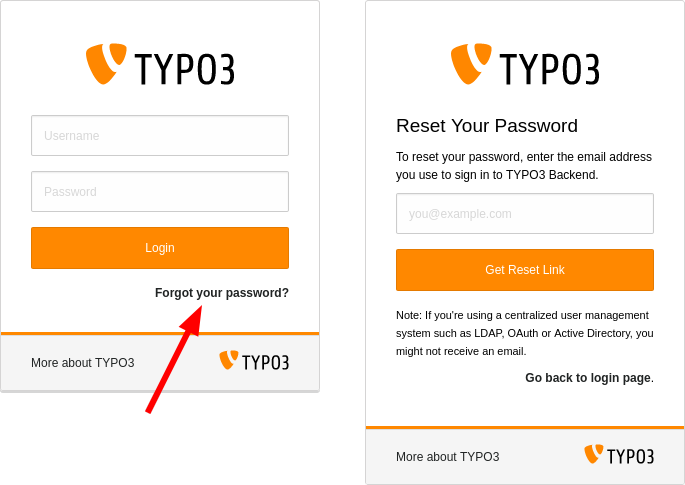
\includegraphics[width=0.6\linewidth]{BackendUserInterface/89513-ProvidePasswordRecoveryForBackendUsers.png}
%	\end{figure}
%
%\end{frame}
%
% ------------------------------------------------------------------------------
